\subsection{dataPreservation}
\label{ss:dataPreservation}
Dieses Package beinhaltet die beiden Klassen dieses Projekts, welche sich mit dem Schreiben und Lesen von Dateien auseinandersetzen. Die Loader Klasse ist hierbei zur Speicherung / zum Laden des Spiels gedacht, w"ahrend sich die Logger Klasse mit dem Schreiben in die Log-Datei besch"aftigt. 

\begin{figure}
	\centering
	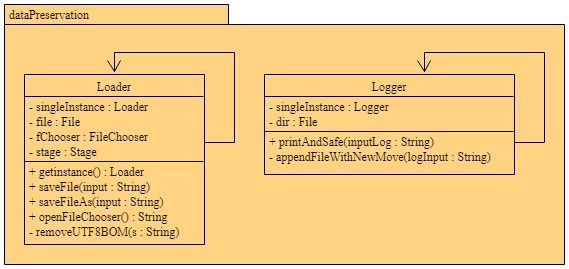
\includegraphics{pics/dataPreservationPackage}
	\caption{UML-Darstellung des dataPreservation packages}
	\label{fig:dataPreservationPackage}
\end{figure}
o
\paragraph{Singleton-Muster}
\label{par:singletonMuster}
\emph{Das Singleton-Muster sichert, dass es nur eine Instanz einer Klasse gibt, und bietet einen globalen Zugriffspunkt f"ur diese Instanz.} \cite{Freeman2006}
Der Konstruktor einer Singleton-Klasse ist als private deklariert und kann somit nur innerhalb der Klasse selbst verwendet werden. Es gibt allerdings eine statische Getter-Methode um auf das Objekt zugreifen zu k"onnen. Hierbei ist zu beachten, dass ein neues Objekt nur erstellt wird, wenn vorher \emph{kein} Objekt der Klasse existiert (siehe \ref{lst:singletonMuster}, \nameref{lst:singletonMuster}). Dieses Muster eignet sich hervorragend f"ur Objekte, bei denen es von Nachteil ist, wenn es mehrere Instanzen gibt. 

Die Logger-Klasse ben"otigt nur eine Instanz, da eine gegebene Log-Datei stets erweitert werden soll. Da st"andig von unterschiedlichen Ebenen des Projekts auf diese Instanz zugegriffen wird, ist es sehr praktisch eine statische (globale) Instanz zu halten, welche von allen Klassen problemlos erreicht werden kann. 

Beim Loader gestaltet sich dies "ahnlich. Zwar gibt es nicht allzu viele Zugriffspunkte, allerdings gibt es nur eine globale Instanz der Datei in die gespeichert werden soll. Insbesondere der Fall des Speicherns eines bereits vorher im Spielverlauf gespeicherten Spiels gestaltet sich einfacher, da man bereits die zu "uberschreibende Datei in der statischen Instanz mit verwaltet. 

\begin{lstlisting}[float,style=CodeHighlighting,caption=Singleton-Muster,label=lst:singletonMuster]
public class Singleton {
	private static Singleton singleInstance; 
	
	\\ further instance variables
	
	private Singleton() {}
	
	public static Singleton getInstance() {
		if (singleInstance == null) {
			singleInstance = new SingleInstance(); 
		}
	}
	return singleInstance; 
	
	\\ further methods	
	
}
\end{lstlisting}


\paragraph{Logger}
\label{par:logger}
Die Logger-Klasse h"alt, wie im Paragraph \nameref{par:singletonMuster} bereits beschrieben, ein Feld namens \emph{singleInstance} vom Typ der Klasse \emph{Logger} um die einzige globale Instanz zu verwalten. Diese wird im Konstruktor entsprechend gesetzt (genau wie in Listing \ref{lst:singletonMuster}, \nameref{lst:singletonMuster}). 

Au"serdem besitzt die Klasse ein Feld mit dem Datentyp \emph{File} um eine Datei zu speichern beziehungsweise zu erweitern. Im Konstruktor wird diese mit einem Konstanten beschrieben, welche eine Datei im Ordner \emph{./dataOutput/logFile.txt} referenziert. Die Datei ist allerdings nicht \emph{final} und kann "uber diverse Setter entsprechend ver"andert werden. 

Um eine Nachricht auf der Konsole auszugeben, sowie in eine Datei zu schreiben, wird die Methode \emph{printAndSafe(...)} verwendet (siehe \ref{lst:logger_printAndSafe}, \nameref{lst:logger_printAndSafe}). Die Methode verwendet neben dem standard Ausgabestrom eine weitere Hifsmethode um die Nachricht an die Log-Datei anzuh"angen (siehe Listing \ref{lst:logger_appendFileWithNewMove}, \nameref{lst:logger_appendFileWithNewMove}). "Uber ein Flag wird erst einmal "uberpr"uft, ob in einem vorherigen Schreibvorgang der Log-Datei ein Fehler festgestellt worden ist (Zeile 2). Anschlie"send wird eine \emph{try-with-resources}-Anweisung beschrieben. Diese besitzt den Vorteil, dass der Ausgabestrom im Fehlerfall noch geschlossen werden kann. Andernfalls m"usste man dieses Exception-handling "uber einen finally-Block abfangen
\cite{try-with-resources}
. Der Ausgabestrom wird also sicher ge"offnet und der gegebene Text an diesen per \emph{write}-Operation angeh"angt. Im Fehlerfall wird der ein kurzer Hinweis, dass es nicht m"oglich sei eine Logdatei f"ur das laufende Spiel anzufertigen, auf dem standard Fehlerstrom ausgegeben. Anschlie"send wird die Nachricht der ausgel"osten Exception angezeigt. Um in Zukunft nicht erneut in diesen Catch-Block zu laufen wird das Flag \emph{loggingPossible} auf \emph{false} gesetzt. 

\paragraph{Loader}
\label{par:loader}
Diese Klasse ist zum Laden und Speichern von Spielst"anden gedacht. Im Konstruktor wird ein Filechooser-Objekt initialisiert. Dieses wird immer wieder verwendet, wenn ein Filechooser-Fenster ge"offnet werden soll um ein neues File-Objekt zu erstellen. In diesem soll der Spielstand gespeichert werden.

\begin{lstlisting}[float,style=CodeHighlighting,caption=Logger - printAndSafe,label=lst:logger_printAndSafe]
public void printAndSafe(String inputLog) {
    System.out.println(inputLog);
    appendFileWithNewMove(inputLog);
}
\end{lstlisting}

\begin{lstlisting}[float,style=CodeHighlighting,caption=Logger - printAndSafe,label=lst:logger_printAndSafe]
public void printAndSafe(String inputLog) {
    System.out.println(inputLog);
    appendFileWithNewMove(inputLog);
}
\end{lstlisting}

\begin{lstlisting}[float,style=CodeHighlighting,caption=Logger - appendFileWithNewMove,label=lst:logger_appendFileWithNewMove]
private void appendFileWithNewMove(String logInput) {
    if (this.loggingPossible) {
        try (Writer outputStream = new BufferedWriter(new FileWriter(this.dir, true))) {
            outputStream.write(logInput + "\n");
        } catch (IOException e) {
            System.err.println(ERROR_DELIMITER 
            	+ "\nThe current game will not have a logfile available:\n"
                + e.getMessage() + "\n" + ERROR_DELIMITER + "\n");
            this.loggingPossible = false;
        }
    }
}
\end{lstlisting}

\subparagraph{Speichern}
Um ein Spiel initial abzuspeichern, ben"otigt man in jedem Fall den beschriebenen Filechooser. Hierzu verwendet man die Methode \emph{saveFileAs}, welche eine Stage initialisiert, den Chooser "offnet und eine weitere Hilfsmethode f"ur den Schreibprozess aufruft \lstref{lst:loader_saveFileAs}. Diese Methode nennt sich \emph{actualSavingProcess} und "offnet einen Ausgabestrom auf den der gegebene Text geschrieben wird \lstref{lst:loader_actualSavingProcess}. Es wird von dem einen Ressourcen-Block Gebrauch gemacht, der den Ausgabestrom selbst bei Abbruch mit einer Exception sicher schlie"st 
\cite{try-with-resources}. 
Neben dem Speichern mit der expliziten Verwendung des Filechooser-Objekts gibt es ebenfalls die Methode {saveFile}, welche die Datei "uberschreibt falls diese bereits vorhanden ist. Falls dies nicht der Fall sein sollte, wird erneut \emph{saveFileAs} aufgerufen. 

\begin{lstlisting}[float,style=CodeHighlighting,caption=Loader - actualSavingProcess,label=lst:loader_actualSavingProcess]
private static void actualSavingProcess(File output, String text) {
    try (PrintWriter outputStream = new PrintWriter(output)){
        outputStream.print(text);
    } catch (FileNotFoundException e) {
        Logger.getInstance().printAndSafe("Could not save file\n" + e.getMessage());
    }
}
\end{lstlisting}

\begin{lstlisting}[float,style=CodeHighlighting,caption=Loader - saveFileAs,label=lst:loader_saveFileAs]
public void saveFileAs(String input) {
    if (null == stage) {
        this.stage = new Stage();
    }
    if (null != this.file) {
        this.fChooser.setInitialDirectory(this.file.getParentFile());
    }
    this.file = fChooser.showSaveDialog(stage);
    if (null == this.file) {
        Logger.getInstance().printAndSafe(Logger.ERROR_DELIMITER
                + "\nUser aborted the saving process\n" + Logger.ERROR_DELIMITER + "\n");
    } else {
        actualSavingProcess(this.file, input);
        Logger.getInstance().printAndSafe("User saved the game as \""
        		 + this.file.getName() + "\" to " + this.file.getPath() + "\n");
    }
}
\end{lstlisting}
